%!TEX root = shrink.tex
\section{Experimental Evaluation}
\label{sec:eval}
\newcommand{\peakS}{Peak-S}
\newcommand{\peakSN}{Peak-SN}
\newcommand{\randSN}{Rand-SN}

Our evaluation has two main goals: (1) Comparing the network energy use of \shrink\ against a network-unaware server consolidation scheme (Section \ref{sec:net-compare}). (2) Quantifying the energy-response time tradeoff achieved by \shrink\ and compare it to the ideal energy response time tradeoff achievable (Section \ref{sec:quantify}).

\begin{figure}[t]
        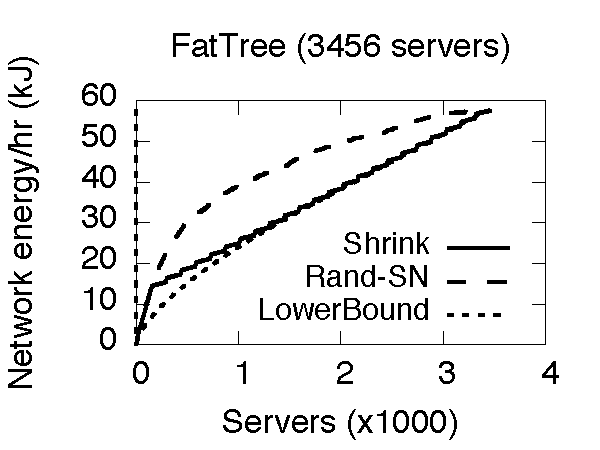
\includegraphics[scale=0.4]{graphs/final/fattree-24.pdf}
                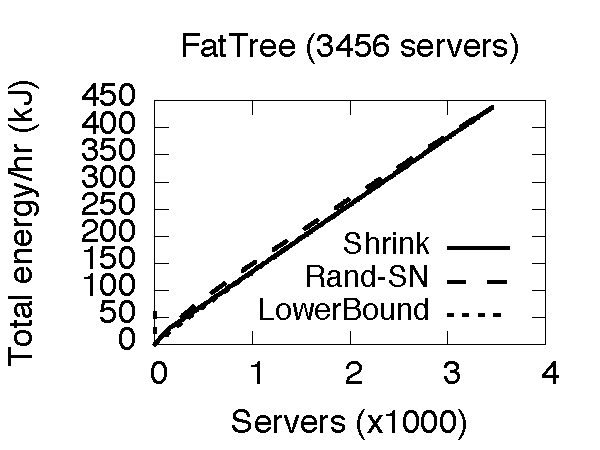
\includegraphics[scale=0.4]{graphs/final/fattree-24-total.pdf}
                        \centering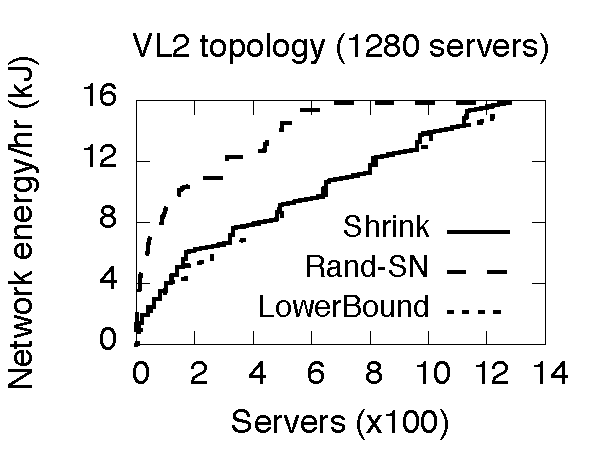
\includegraphics[scale=0.4]{graphs/final/vl2.pdf}
                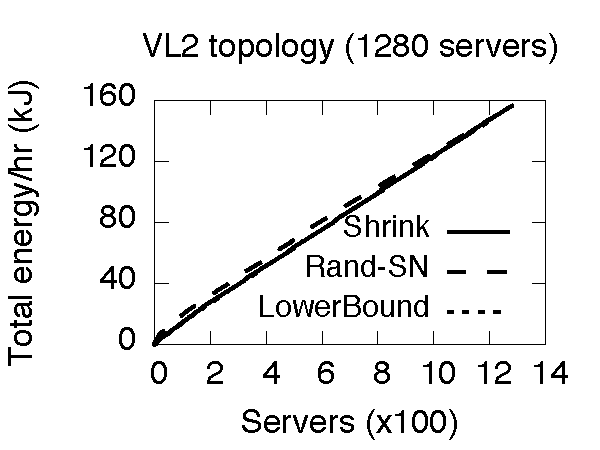
\includegraphics[scale=0.4]{graphs/final/vl2-total.pdf}
\caption{[Numerical computation] \shrink's network energy use is lower than a network-unaware server consolidation scheme \randSN\ by 38\% on FatTree and 42\% on VL2 when one-fourth of the servers are active in each topology.}
\label{fig:fattree}
\end{figure}

\subsection{Comparing network energy use}
\label{sec:net-compare}

\textbf{Schemes compared:}   (1) \emph{\randSN:} \randSN\ selects the set of active servers randomly; it uses the same network consolidation scheme as \shrink.  \randSN\ is used to evaluate the benefit of network-aware server consolidation in \shrink. (2) \emph{LowerBound:} We define lower bounds on the network energy use for a given number of active servers on the FatTree and the VL2 topologies. Our computation of LowerBound for FatTree and VL2 is described in Appendix \ref{sec:netlb}. \randSN\ and LowerBound provide the same per-server bandwidth guarantee to external hosts as \shrink\ does.

\textbf{Topologies:}  We simulate two network topologies:  a 3456-server FatTree topology made of 24-port switches (Cisco Nexus 2224P, 80 Watt, 720 count) \cite{cisco-dc-switches} consuming 80 Watt per switch, and a 1280-server VL2 topology made of 24-port ToR switches (Cisco Nexus 2224P, 80 W, 64 count) \cite{cisco-dc-switches} and 16-port 10 Gigabit core or aggregation switches (Cisco Catalyst 6500, 480 W, 24 count) \cite{catalyst-6500}. We assume all active servers have identical power use (Acer Altos T350 F2, 130W at 60\% utilization \cite{spec}).

\textbf{Results:}  Figure \ref{fig:fattree} presents our results.
%compares \shrink\ against \randSN\ and the lower bounds on network energy use for the simulated topologies.
The relative difference between \shrink\ and \randSN\ reduces as the number of active servers increases. 
When 25\% and 50\% of servers are active, \shrink's network energy use is lower than \randSN\ by 38\% and 26\% respectively on FatTree and 42\% and 35\% respectively on VL2. 
When 25\% and 50\% of servers are active, \shrink's network energy use higher than LowerBound by 9\% and 2\% respectively on FatTree and by 13\% and 7\% respectively on VL2. 
These findings show that \shrink's network-aware server consolidation reduces the network energy use over network-unaware server consolidation schemes and gives network energy savings close to the lower bound.
When 25\% and 50\% of servers are active, \shrink's \emph{total} energy use is lower than \randSN\ by 9\% and 5\% respectively on FatTree and 10\% and 7\% respectively on VL2. 
Thus, \shrink's network-aware server consolidation is effective in reducing aggregate \cdc\ energy use as well. 

%Considering scenarios where at least one-fifth of servers are active, \shrink\ uses up to 39\% less network energy on FatTree and up to 45\% less energy on VL2 compared to the network-unaware scheme, \randSN. 


\begin{figure*}
        \centering
        \subfigure[Mean]{\label{fig:pe-mean}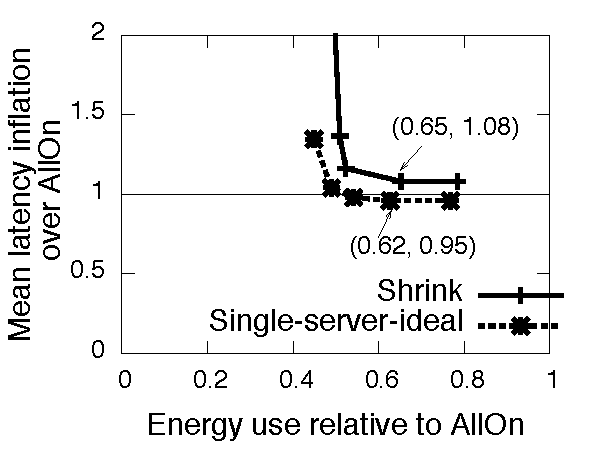
\includegraphics[scale=0.47]{graphs/final/mean.pdf}}
         \subfigure[95-th percentile]{\label{fig:pe-95}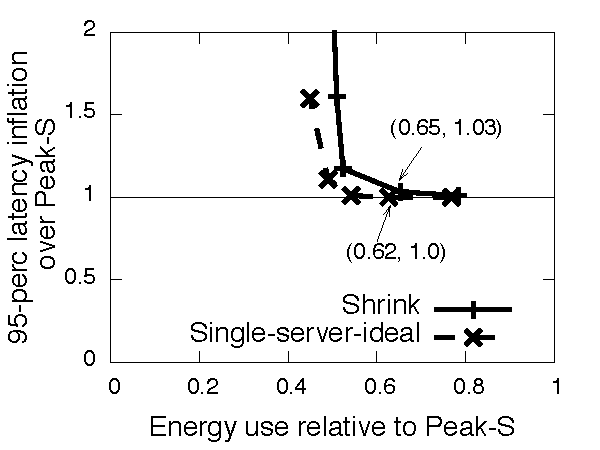
\includegraphics[scale=0.47]{graphs/final/perc95.pdf}}	       \subfigure[99-th percentile]{\label{fig:pe-99}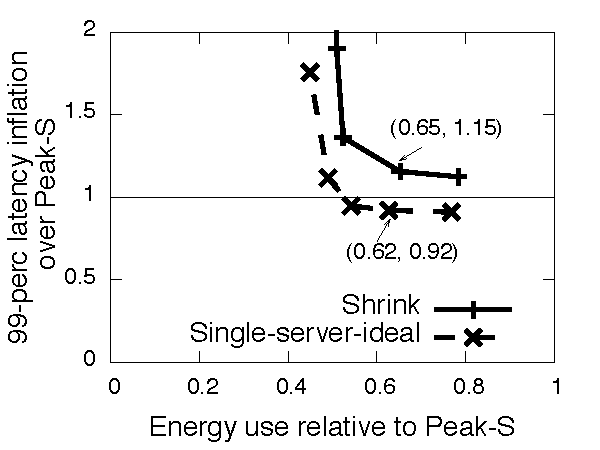
\includegraphics[scale=0.47]{graphs/final/perc99.pdf}}	
        \caption{Server consolidation (Section \ref{sec:ec2}):  \shrink's reduces energy over \peakS\ with a small response time inflation. In Figure \ref{fig:pe-mean}, \shrink's energy use is 0.65$\times$ of \peakS\ and its mean response time is 1.08$\times$ of \peakS; Single-server-ideal's energy use is 0.62$\times$  of \peakS\ and its mean response time is 0.95$\times$ of \peakS.}
        \label{fig:pe}
\end{figure*}

\subsection{Quantifying energy-response time tradeoff}
\label{sec:quantify}
\vspace{-0.1in}
\subsubsection{Experiment setup}
\label{sec:setup}
\textbf{Akamai dataset:} Our evaluation uses content access traces from an Akamai datacenter. The traces include all requests received at a datacenter with 24 servers for a week in December 2013. We restricted our data collection to a small datacenter as we did not have the resources to experiment with traces from a significantly larger datacenter. Our anonymized traces include several major types of traffic observed in a CDN such as video, social media and other web traffic. Each anonymized log entry includes among other fields, the request timestamp, content URL, size of requested content, actual number of bytes sent and IP address of the user. Overall, the traces contain more than 2 billion requests generating nearly 200 TB of network traffic.

\textbf{Testbeds:} We use prototype-based experiments (on EC2 and Emulab) and trace-based experiments. Our experiment on EC2 evaluates the energy-response time tradeoff due to server-only consolidation. As we do not have control over network topology on EC2, we use Emulab to evaluate the response time inflation due to both server and network consolidation. Finally, we conduct larger-scale trace-based experiments on a simulator.






%\begin{figure}[t]
%        \centering
%        \begin{subfigure}{0.24\textwidth}
%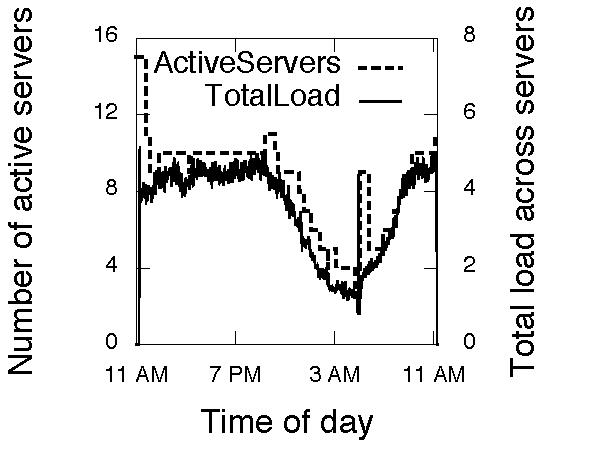
\includegraphics[scale=0.4]{graphs/final/num-servers.pdf}
%\caption{}
%\label{fig:num-servers}
%        \end{subfigure}
%        \begin{subfigure}{0.24\textwidth}
%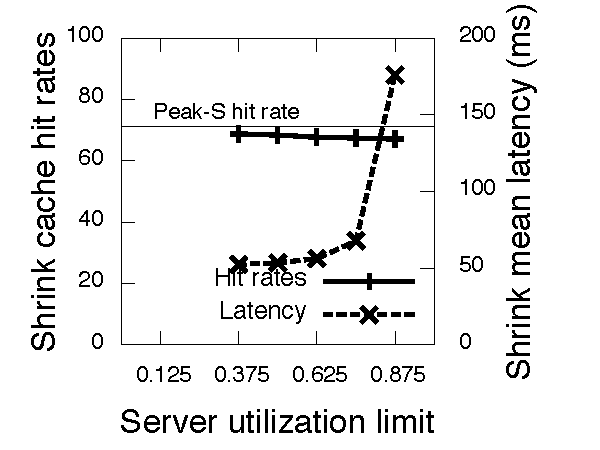
\includegraphics[scale=0.4]{graphs/final/hit-rate.pdf}
%\caption{}
%\label{fig:hitrate}
%        \end{subfigure}
%        \caption{[EC2] \shrink\ adapts the number of active servers based on \cdc\  load to reduce energy over \peakS. Cache hit rates and mean response time for \shrink\ and \peakS.}
%\end{figure}


%\centering
%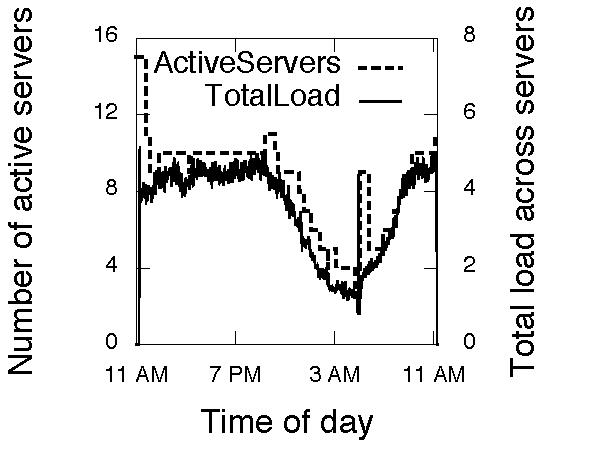
\includegraphics[scale=0.6]{graphs/final/num-servers.pdf}
%\caption{[EC2] \shrink\ adapts the number of active servers based on \cdc\  load to reduce energy over \peakS.}
%\label{fig:num-servers}
%\end{minipage}
%\hspace{0.5cm}
%\begin{minipage}{0.3\textwidth}
%\centering
%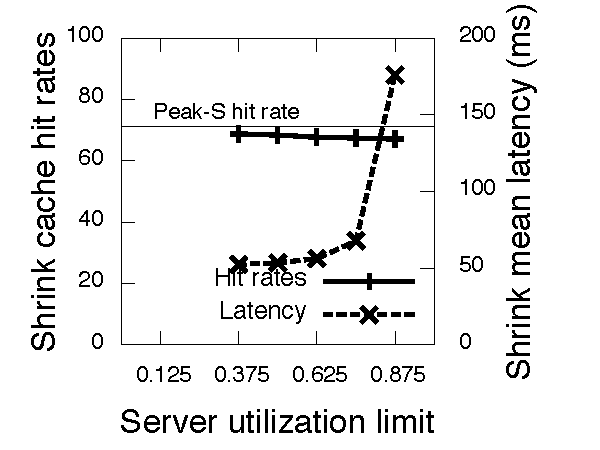
\includegraphics[scale=0.6]{graphs/final/hit-rate.pdf}
%\caption{[EC2] Cache hit rates and mean response time for \shrink\ and \peakS.}
%\label{fig:hitrate}
%\end{minipage}
%\hspace{0.5cm}
%\begin{minipage}{0.3\textwidth}
%\centering
%	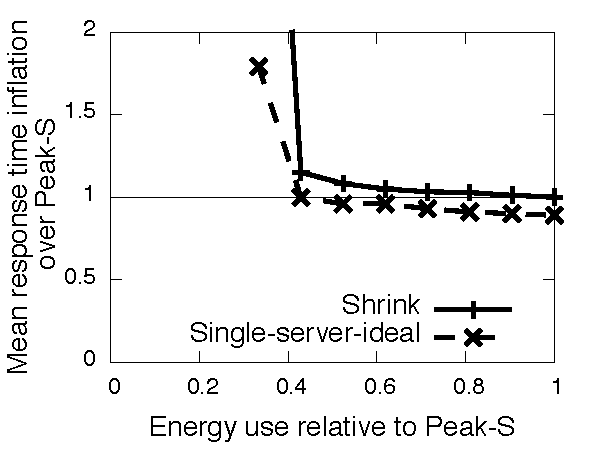
\includegraphics[scale=0.55]{graphs/final/emulab-mean.pdf}
%	\caption{[Emulab] Network and server consolidation: For an 15\% increase in mean response time, \shrink\ reduces energy use by 57\% over \peakS.}
%	\label{fig:pe-mean-2}
%
%\end{minipage}
%\end{figure*}

%
%\begin{figure*}
%\begin{minipage}{0.3\textwidth}
%\centering
%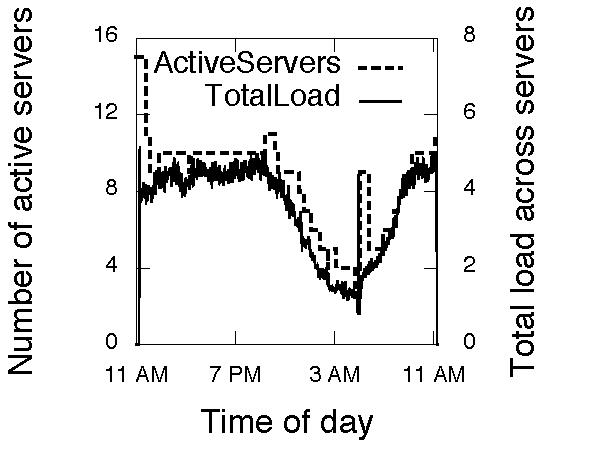
\includegraphics[scale=0.6]{graphs/final/num-servers.pdf}
%\caption{[EC2] \shrink\ adapts the number of active servers based on \cdc\  load to reduce energy over \peakS.}
%\label{fig:num-servers}
%\end{minipage}
%\hspace{0.5cm}
%\begin{minipage}{0.3\textwidth}
%\centering
%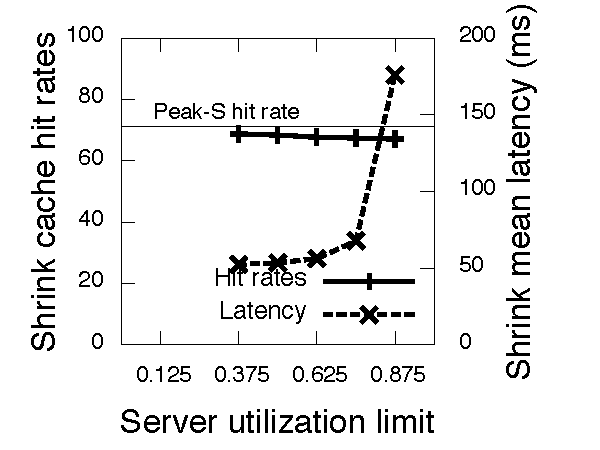
\includegraphics[scale=0.6]{graphs/final/hit-rate.pdf}
%\caption{[EC2] Cache hit rates and mean response time for \shrink\ and \peakS.}
%\label{fig:hitrate}
%\end{minipage}
%\hspace{0.5cm}
%\begin{minipage}{0.3\textwidth}
%\centering
%	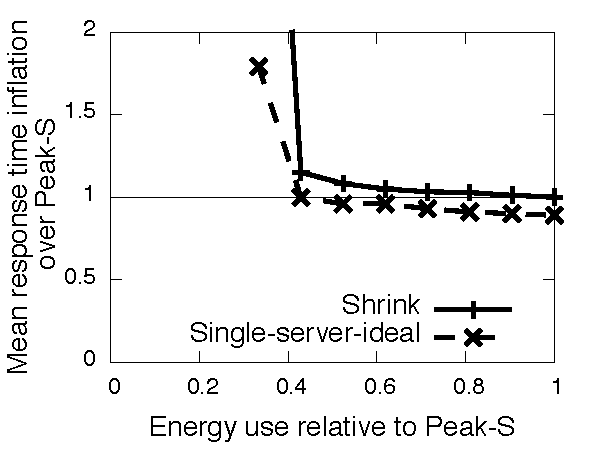
\includegraphics[scale=0.55]{graphs/final/emulab-mean.pdf}
%	\caption{[Emulab] Network and server consolidation: For an 15\% increase in mean response time, \shrink\ reduces energy use by 57\% over \peakS.}
%	\label{fig:pe-mean-2}
%
%\end{minipage}
%\end{figure*}


\textbf{Schemes compared:} We compare \shrink\ against \emph{\peakS} and \emph{Single-server-ideal}. \peakS\ represents a baseline in which a \cdc\ operator does not use consolidation to reduce energy use, i.e., it keeps all servers and switches active.

Single-server-ideal is a computation of the ideal energy-response time curve, unachievable by any real system. The points on this curve are obtained by varying the utilization $u$ up to which any server can be loaded. For a given $u$, the response time of Single-server-ideal for a given metric is equal to the measured load-vs.-response time curve of a single server for the same metric at the same utilization. For the same utilization $u$, any distributed system will have a higher response time because workload dynamics, load imbalance and non-steady state cache behavior; these factors are ignored by Single-server-ideal. Our single server measurements are done with a representative workload in the respective experimental environment, EC2 or Emulab, with emulated client-to-server delay and server-to-origin delay. 

%taken to be response of a single server in steady-state at the same utilization. In doing so, we assume that the response time of the entire \cdc\ at a given average utilization is the same as that of a single server  at the same utilization. 

For Single-server-ideal, we compute the set of servers and switches in each time interval that minimizes the total energy use as follows. Based on four inputs -- $u$, the total load in each time interval, the number of server transitions allowed, and the power model of each server --, we use a dynamic programming algorithm to compute the total energy use of servers and the number of active servers in each time interval. The number of transitions is equal to one on-off server transition/server/day or the same number of transitions as \shrink\ in that experiment, whichever is higher. The ideal network energy use for the tree topology we experiment with (Section \ref{sec:emulab}) is computed based on the number of active servers in each time interval. The set of active servers are selected in a left-to-right order; for each active server, we select the switches on the path to the root. The set of switches selected across all active servers is the set that optimizes network energy use.

%Single-server-ideal is a computation of the ideal energy-response time curve. In our computation, we assume that the utilization-vs.-response time curve for the entire \cdc\  is the same as that of a single server system at the same utilization, which is in steady state and has an infinite cache. 
%The response time of Single-server-ideal is \emph{ideal}, as discussed in Section \ref{sec:analysis}. For our computation, we obtained the utilization-vs.-response time curve for a single server by measuring response time metrics at varying request rates and using a cache size large enough so that steady state response times can be measured without exhausting the cache.
%
%The energy calculation for Single-server-ideal assumes prior knowledge of the total load in each time interval and the number of server transitions allowed. We allow Single-server-ideal to make one on-off server transition/server/day or the same number of transitions as \shrink\ in that experiment, whichever is higher. Based on these inputs, we use a dynamic programming algorithm \cite{mathew12} to compute the total energy use of servers and the number of active servers in each time interval.  The network energy use for the tree topology we experiment with (Section \ref{sec:emulab}) is computed as follows: For each active server, we select the switches on the path to the root. The set of switches selected across all active servers is the set that optimizes network energy use.



\subsubsection{Prototype-based experiments: server\\ consolidation}
\label{sec:ec2}
\vspace{-0.1in}
This experiment quantifies the energy-response time tradeoff due to server consolidation on EC2. Our EC2 testbed consists of 15 servers, 15 clients and 4 origin servers running on independent m3.xlarge instances (4 core, 15 GB RAM, 40 GB$\times$2 SSD), all in the same datacenter. Our origin server is a trivial Apache Tomcat application that dynamically generates the requested content. We emulate a 60 ms RTT between origin servers and \cdc's servers, and a 10 ms RTT between client and server machines. We configured each server to use an 8 GB memory cache and a 30 GB cache on each SSD. 

Our workload consists of a 24-hour duration of the trace.  We selected one-eighth of the content randomly from the trace but sped up the trace by 8$\times$ to send those requests over a 3-hour duration. Thus, we  maintain approximately the same load on the servers. We use a short pre-shutdown wait interval $W =$ 10 min for \shrink\ because our workload is a sped up by $8\times$.

%
We calculate the energy savings relative to \peakS\ as per Equation \ref{eq:benefit}; the ratio of the idle to peak energy use of servers, $I$ equals 0.5 \cite{barroso2007case}. \peakS\ uses 15 servers in this experiment. We have conservatively chosen the number of servers in \peakS\ to be much less than the number of servers in the Akamai datacenter itself so as not to overestimate the energy savings. 



We evaluate \shrink\ in terms of three response time metrics --  mean, 95-percentile, 99-percentile. 
To provide a utilization-vs.-response time curve $F(.)$ to \shrink\ for each metric, we take the first approach discussed in Section \ref{sec:utilization-vs-responsetime}. The function $F(.)$ for each metric is equal to the measured utilization vs. response time curve of a single server with an inefficiency factor $\rho = 0.2$.  Based on $F(.)$ for each metric, we specify response times $F(u)$ to \shrink\ for values of $u$ from 0.375 to 0.875 at intervals of 0.125 across different runs. 

%, which is much less than the number of servers in the Akamai datacenter itself. we have made this choice not to overstate the energy savings.


Figure \ref{fig:pe} compares the response time and the energy use of \shrink\ relative to \peakS\ for the mean, the 95-th percentile and the 99-th percentile of response times. \shrink\ reduces energy use by 35\% over \peakS\ while inflating the mean, the 95-th percentile and the 99-th percentile by 8\%, 3\% and 15\% respectively. 
To explain the difference between \peakS\ and \shrink, consider Figure \ref{fig:ec2-other} (left)  which shows the aggregate load and the number of servers from one of the runs of the system. \shrink\  adapts the number of active servers based on load in the system keeping only 3 servers active when the load is the lowest, but \peakS\ always keeps 15 servers active and hence has a higher energy use. This result implies that an operator for which these inflations are tolerable, e.g., they do not cause an SLA violation, can achieve the corresponding energy savings as well. 




%Single-server-ideal does achieve a better energy-response time tradeoff than \shrink.  First, the energy-response time curve for Single-server-ideal is computed assuming that the response time for a given server utilization limit is equal to the response time of a single server in steady state at the same utilization. The response time for any real system, including \shrink, will be higher due to several reasons such as imperfect load balancing and non-steady state cache behavior. 




Does  an increase server load or a decrease in cache hit rates cause a greater impact on \shrink's response time over \peakS? 
In Figure \ref{fig:ec2-other} (right) the x-axis shows the server utilization limit $U$ computed by \shrink's consolidation algorithm (Section \ref{sec:serverconsolidation}) and y-axes show corresponding the  hit rates and the mean response time of \shrink. \shrink's  hit rates are lower than \peakS\ but the decrease is less than 7\% across all utilizations. 
Thus, the response time inflation due to a decrease in hit rates is likely to be small. A small reduction in hit rates is not surprising given that the Zipf exponent for the Akamai trace is 0.8 as per our calculations, and our model in Section \ref{sec:analysis} has suggested that  consolidation reduces hit rates by a small fraction for for real workloads with a high skew in content popularity.  We find that mean response times increase sharply at  a high server utilization limit, e.g. $U=0.875$, which is likely due to an increase in server load. To summarize, there is a small response time inflation due to a decrease in hit rates but severe inflation occurs at high server utilization limits, and is likely due to an increase in server  load.


Comparing \shrink\ with Single-server-ideal, in Figure \ref{fig:pe-mean}, \shrink's energy use is 0.65$\times$ of \peakS\ and its mean response time is 1.08$\times$ of \peakS; Single-server-ideal's energy use is 0.62$\times$  of \peakS\ and its mean response time is 0.95$\times$ of \peakS.  
There are two reasons that explain the gap between \shrink\ and Single-server-ideal. First, Single-server-ideal ignores several factors that increase response time of any distributed system such as workload dynamics, load imbalance and non-steady state cache behavior. Second, \shrink\ waits for the pre-shutdown wait interval to see if a decrease in load persists before turning servers off. But, in our calculation, Single-server-ideal knows the load for the entire experiment beforehand and hence it can shutdown servers sooner than \shrink\ and save more energy.

%An implication of our findings is that a simple random load balancing policy effectively avoids load hotspots and ensures only a small decrease in cache hit rates even as energy optimization schemes vary the number of active servers in a \cdc.
\begin{figure}
\centering
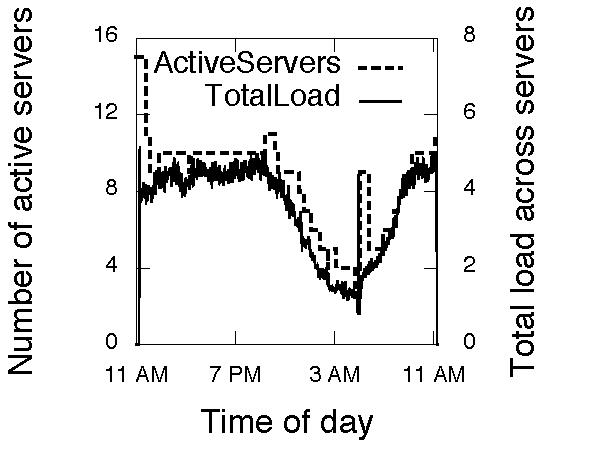
\includegraphics[scale=0.4]{graphs/final/num-servers.pdf}
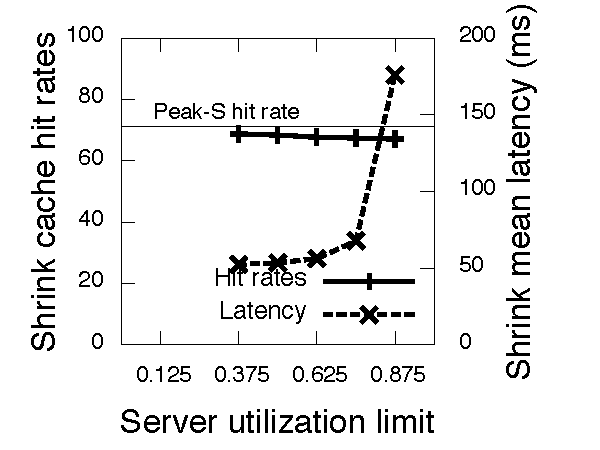
\includegraphics[scale=0.4]{graphs/final/hit-rate.pdf}
\caption{Server consolidation (Section \ref{sec:ec2}): [Left] \shrink\ adapts the number of active servers based on \cdc\  load to reduce energy over \peakS. [Right] Cache hit rates and mean response time for \shrink\ and \peakS.}
\label{fig:ec2-other}
\end{figure}

\subsubsection{Prototype-based experiments: server \& network consolidation}
\label{sec:emulab}

\begin{figure}
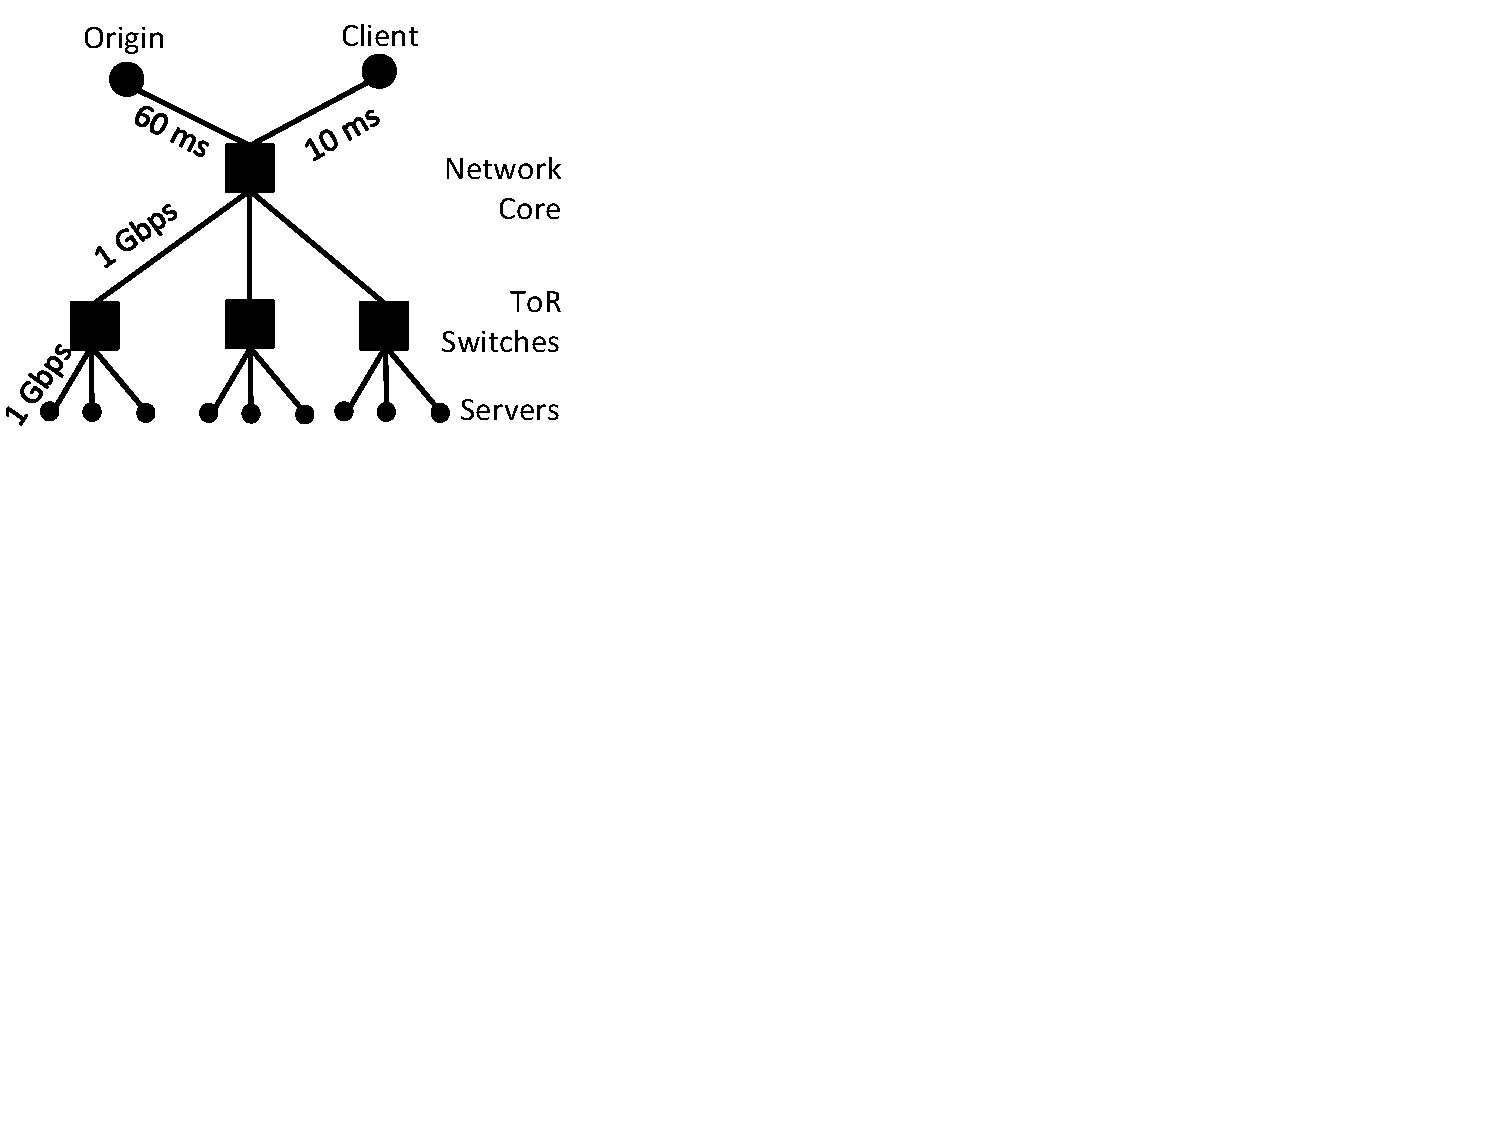
\includegraphics[scale=0.35]{figures/emulab-topo.pdf}
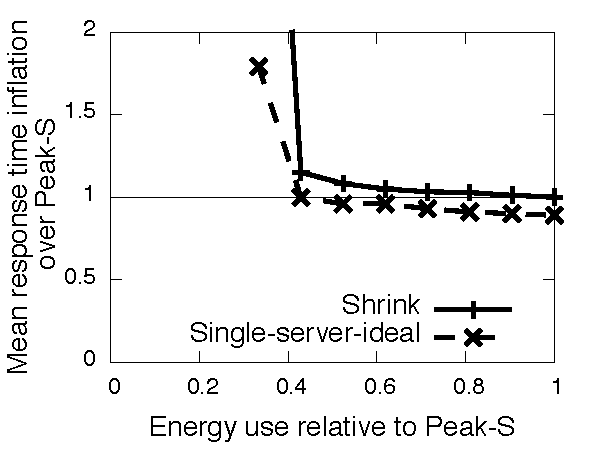
\includegraphics[scale=0.5]{graphs/final/emulab-mean.pdf}
\caption{Network and server consolidation (Section \ref{sec:emulab}): [Left] Emulab topology for the experiment. [Right] Compared to \peakS, \shrink\ has a 15\% higher response time but a 57\% lower energy use.}
\label{fig:emulab}
\end{figure}

We use Emulab to evaluate the energy-response time tradeoff when both server and network consolidation are being performed. For our experiment, we configure a tree topology with 1 Gbps links as shown in Figure \ref{fig:emulab} (left). 
In this topology, the ToR switches have 4 ports, and the core switch has at least 4 ports. Accordingly,  we calculate energy use of switches based on the power use of 4-port switch (Netgear GS105), which is 14.4 W \cite{netgearGS105}. The energy use of servers is computed using the same function as in the previous experiment. Our workload consists of a 1-hour duration of the trace containing requests for one-eighth of the content selected randomly.

Figure \ref{fig:emulab} (right) compares schemes in terms of the mean response times.  Across different runs that vary specified mean response times, \shrink\ uses between 2 and 9 servers; \peakS\ uses 9 servers.  We discuss the case when \shrink\ uses 3 servers so that only one of the ToR switches are being used as a result of network consolidation. In this case, the peak utilization of the link between the ToR and the core switch increased up to 76\% during the experiment, which is nearly three times higher than the peak link utilization for \peakS. Despite this increase, \shrink's response time is only 15\% higher than \peakS, while its network energy use is 50\% lower and the overall energy use is 57\% lower than \peakS\ (second point from the left in Figure \ref{fig:emulab} (right)). This result shows that both network and server consolidation can be performed with a small performance impact in \cdc s. Finally, we note that the difference between Single-server-ideal and \shrink\ is consistent with the difference between them in our experiment with server-only consolidation,, e.g., for the same energy savings as \shrink\ (= 57\%), \shrink's response time is 15\% more than Single-server-ideal.



%\begin{figure*}
%\begin{minipage}{0.3\textwidth}
%\centering
%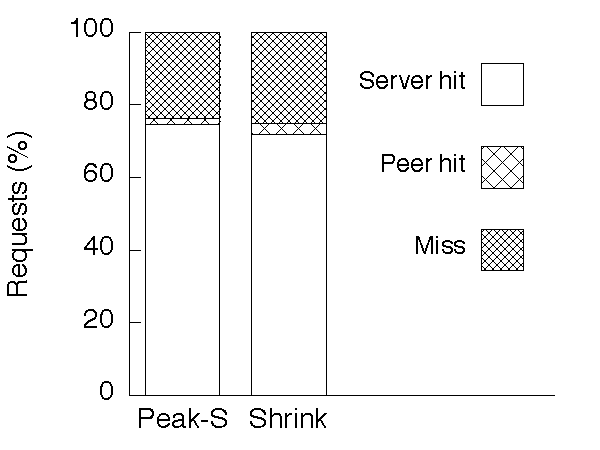
\includegraphics[scale=0.5]{graphs/final/sim-hitrate.pdf}
%\caption{[Simulator] \shrink\ increases miss rates by 1.5\% over \peakS\ over a one-week long trace showing that energy optimization in \cdc s hurts cache hit rates by a small margin. }
%\label{fig:sim-hitrate}
%\end{minipage}
%\hspace{0.5cm}
%\begin{minipage}{0.3\textwidth}
%\centering
%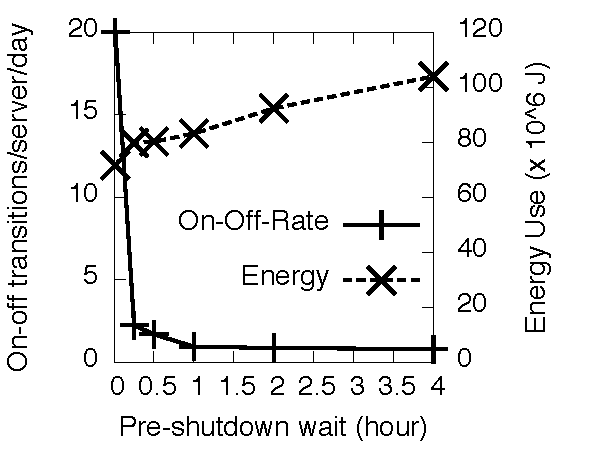
\includegraphics[scale=0.5]{graphs/final/onoff.pdf}
%\caption{[Simulator] Pre-shutdown wait interval ($W$) between 30 min \& 1 hour keeps on-off transition rate close to 1/server/day and with only a small increase in energy use over $W$ = 1 min.}
%\label{fig:sim-onoffrate}
%\end{minipage}
%\hspace{0.5cm}
%\begin{minipage}{0.3\textwidth}
%\centering
%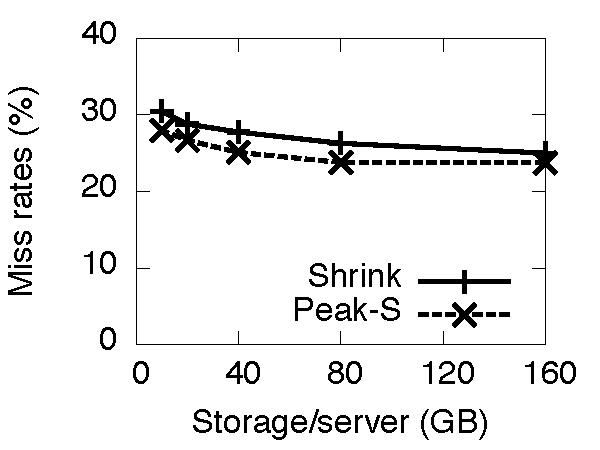
\includegraphics[scale=0.5]{graphs/final/storage.pdf}
%\caption{[Simulator] Difference between miss rates for both \shrink\ and \peakS\ is consistent despite variations in storage capacity.}
%\label{fig:sim-storage-vs-hitrate}
%\end{minipage}
%\end{figure*}

\subsubsection{Trace-based experiments}
\label{sec:simulation}
%The following are the goals of our trace-based experiments: (1) Quantify energy savings of server consolidation over the complete duration of the trace for a given server utilization limit expected to cause a small impact in response time.
%(2) Evaluate the potential benefit of cooperative caching among servers in a \cdc\ assuming that a cache-coordination protocol with a much smaller overhead can be developed in future. 
%(3) Quantify the tradeoff between energy savings and reliability by varying the pre-shutdown wait interval $W$.
%(4) Analyze the sensitivity of hit rates to a server's storage capacity.

\textbf{Methodology:} We conduct experiments for a \cdc\ with 16 servers for the week-long Akamai trace. The capacity of each server is defined in terms of network traffic it can support. The rate of network traffic generated by a request is a constant equal to the client bandwidth reported in the Akamai trace. To be able to fit the simulator process in the memory on our machine (32 GB), we filtered requests for one-eighth of the content from the trace. Accordingly, we scale down  the capacity of each server to be 150 Mbps, and the cache size per server to be 150 GB. Since trace-based experiments do not provide an accurate estimate of response times, we used a fixed server utilization limit $U$ = 0.65 for our experiments, which is expected to cause a small response time inflation (Figure \ref{fig:ec2-other} (right)). 
The cache hit rates of our simulator's LRU caching and Squid differ by less than 2\% for the same workload and cache size. 


\begin{figure}
\centering
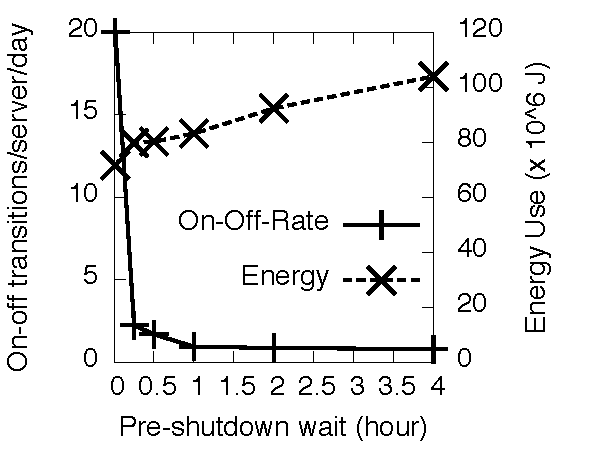
\includegraphics[scale=0.4]{graphs/final/onoff.pdf}
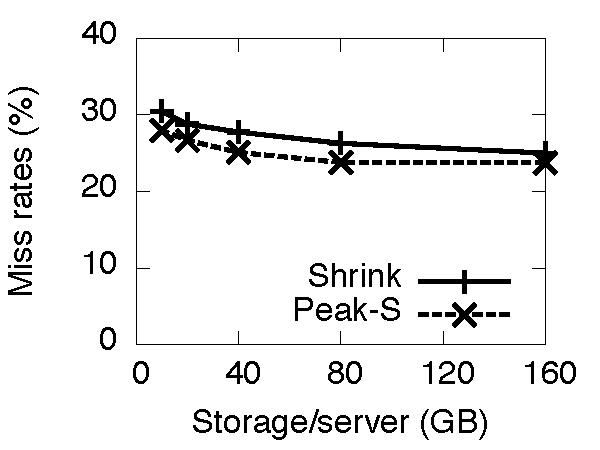
\includegraphics[scale=0.4]{graphs/final/storage.pdf}
\caption{[Simulator] [Left] Pre-shutdown wait interval between 30 min \& 1 hour keeps on-off transition rate close to 1/server/day. [Right] Comparison of miss rates for varying amounts of storage.}
\label{fig:sim-onoffrate}
\end{figure}
\textbf{Impact on hardware reliability:} Figure \ref{fig:sim-onoffrate} (left) shows the rate of on-off transitions per server and the corresponding energy savings is achievable. We find that a short pre-shutdown wait interval $W$ = 1 min hurts hardware reliability by increasing the rate of server transitions to more than 20/server/day. On the other hand, a  high $W$ = 4 hours reduces server transition rate to 0.81/server/day, but increases energy use by nearly 45\% over $W$ = 1 min.  The sweet spot for pre-shutdown wait interval is between 30 min to 1 hour, where increase in energy use over $W$ = 1 min is between 12\% and 15\%  but most of the reduction in on-off transition rates can still be achieved.

\textbf{Storage vs. cache miss rates:} To determine the sensitivity of miss rates to available storage, we evaluate \peakS\  and \shrink\ for varying amount of storage from 10 GB/server to 160 GB/server and present results in Figure \ref{fig:sim-onoffrate} (right). We remark that we have scaled down the CDN trace and hence the storage by a 8$\times$ factor, i.e., we would have provisioned 1.28 TB storage instead of 160 GB if we were to experiment with the full trace.  As storage reduces, the miss rates increase as expected. But, the relative difference between miss rates for both \shrink\ and \peakS\  remains nearly the same even on reducing the storage to 10 GB, e.g., \shrink's miss rates are 10.3\% higher than that of \peakS\  for 160 GB storage and are 9.6\% higher than that of \peakS\  for 10 GB storage. Thus, we conclude that server consolidation schemes are expected to increase datacenter miss rates by a small fraction within the range of storage typically available on server-class machines. 

\textbf{Cooperative caching benefit:} We evaluate the potential benefit of cooperative caching among servers in a \cdc\ assuming that a cache-coordination protocol with a much smaller overhead can be developed in future. The hit rates at cache peers  are 1.65\% for \peakS\  and 3.02\% for \shrink, which suggests that cooperative caching among datacenter servers, if implemented efficiently, could reduce the impact of energy optimization schemes by a small margin. 
%We present other results from trace-based experiments here. 
%(1) Over a one-week long trace. \shrink\ provides 37\% energy savings over \peakS. (2) 

%\textbf{Energy savings and cache hit rates:}
%We have compared the energy use of \shrink\ against other schemes over a one-week long trace. \shrink\ provides 37\% energy savings over \peakS\ in that experiment. We skip a detailed discussion of the results noting that energy use of other schemes are qualitatively similar to that observed in the experiment on EC2.
%
%Figure \ref{fig:sim-hitrate} compares the server hit rates, peer hit rates and miss rates. We make two key observations from this graph. First, there is less than 1.5\% difference in miss rates between \shrink\ and \peakS\  scheme, which supports our earlier observation in prototype-based experiments that \shrink's energy optimization does cause a significant increase in miss rates.  Second, we note that peer hit rates are 1.65\% for \peakS\  and 3.02\% for \shrink, which suggests that cooperative caching among datacenter servers could reduce the impact of energy optimization schemes by a small margin. Implementing a cooperative caching scheme with a low overhead is a topic of future work.




\eat{
%\begin{figure}
%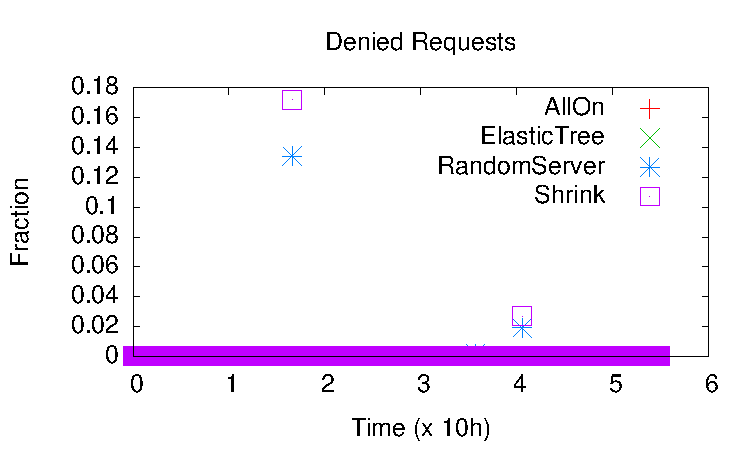
\includegraphics[scale=0.6]{graphs/server-logs/denied.pdf}
%\caption{Fraction of requests that are denied. \peakS\  scheme denies no requests throughout the experiment, whereas other schemes have a non-zero denied requests in a few time intervals. Both intervals  where requests are denied happened in cases of sudden spikes in load during night time.}
%\label{fig:sim-availability}
%\end{figure}

Figure \ref{fig:sim-availability} shows the fraction of requests that are denied due to server unavailability. Each data point represents denied requests in a 5-min interval. We find that the \peakS\  scheme has no denied requests throughout the experiment, i.e., it has 100\% availability. \shrink\ also has 100\% in all time intervals, except for two. Further analysis showed that both these intervals occured in late-night hours between 2 AM and 4 AM when there was unexpected spike in load that was 4 times the expected load in that interval. The active servers at that time did not sufficient enough resources to handle the request load. Thus, there was a brief period of unavailability until more servers could be turned on. That server unavailability is near-perfect an encouraging sign for deploying server consolidation, but also shows that energy-optimizing schemes make a \cdc\ less tolerant to highly unpredictable increase in load. A possible way to reduce the impact of such unavailability is to keep servers in a sleep state instead of completely turning them off so that they can be turned on quickly if necessary. 
}

%\begin{figure}
%\centering
%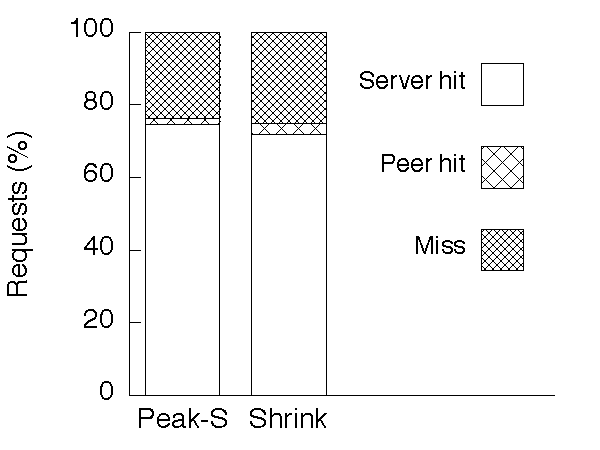
\includegraphics[scale=0.6]{graphs/final/sim-hitrate.pdf}
%\caption{[Simulator] \shrink\ increases miss rates by a small margin of 1.5\% over \peakS\ over a one-week long trace showing that energy optimization in \cdc s hurts cache performance by a small margin. }
%\label{fig:sim-hitrate}
%\end{figure}



%\begin{figure}
%\centering
%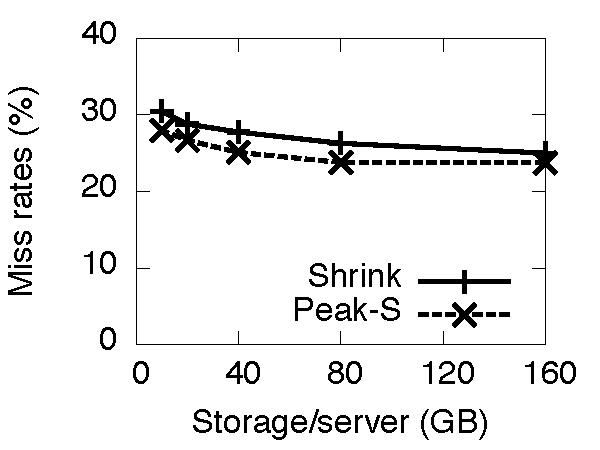
\includegraphics[scale=0.6]{graphs/final/storage.pdf}
%\caption{}
%\label{fig:sim-storage-vs-hitrate}
%\end{figure}



